\documentclass[12pt, letterpaper]{article}

\makeatletter
\newcommand{\@BIBLABEL}{\@emptybiblabel}
\newcommand{\@emptybiblabel}[1]{}
\makeatother
\usepackage[hidelinks]{hyperref}
\usepackage{enumitem}
\usepackage{fullpage}
\usepackage[english]{babel}
\usepackage[utf8x]{inputenc}
\usepackage{amsmath}
\usepackage{amssymb}
\usepackage{graphicx}
\usepackage[colorinlistoftodos]{todonotes}
\usepackage[linesnumbered]{algorithm2e}
\usepackage{tabularx}
\usepackage{url}
\usepackage{hyperref}
\hypersetup{colorlinks=true}
\usepackage[margin=1in]{geometry}
\usepackage[english]{babel}
\usepackage{mathtools}
\usepackage{booktabs}
\usepackage{physics}
\usepackage{float}
\usepackage{tabularx}
\newcolumntype{C}{>{\centering\arraybackslash}X}

\begin{document}
\title{CS 7650 Midterm}
\author{Instructor: Dr. Wei Xu \\ TAs: Mounica Maddela, Nathan Vaska, and Sarah Wiegreffe}
\date{}
\maketitle

\section{Word Embeddings}

The \textsc{Word2Vec} algorithm revolutionized the field of NLP by providing a high-quality, but cheaply computable means for producing continuous vector representations of words learned from a large, unlabelled corpus. Here, we will investigate the objectives used in the \textsc{Word2Vec} algorithm. This question may require you to refer to Chapters 14.5, 14.6 of the Eisenstein readings. \\

Here is a sentence for which the algorithm will make a prediction for the missing word. The word embedding for each word in the context has been given.

\begin{table}[h!]
    \centering
    \begin{tabular}{|ccc|}
    \toprule
    \textbf{Index Position} & \textbf{Word} & \textbf{Embedding} \\
    \midrule
    0 & the & $[2,1]$ \\
    1 & quick & $[3,2]$ \\
    2 & brown & $[-2,0]$ \\
    3 & ? & ?\\
    4 & jumped & $[5,-1]$\\
    5 & over & $[2,-3]$\\
    6 & the & $[2,1]$\\
    7 & lazy & $[-3,-1]$\\
    8 & dog & $[1,2]$\\
    
    \bottomrule
    \end{tabular}
    \caption{Word Embeddings for the Input Sentence.}
\end{table}

\begin{enumerate}
    \item Compute the Continuous Bag-of-Words (CBOW) vector representation of the missing word for a context window $h$ of size 3. Show your work.

    \item We've subset the vocabulary down to the words in Table \ref{tab:vocab}. Fill in the scores of each word being the missing word in Table \ref{tab:vocab}. Use the base-2 exponent and round to 2 decimal places.\\
    Hint: use dot products for this, not traditional vector-space similarity.
    
\begin{table}[h!]
    \centering
    \begin{tabular}{|c|c|c|c|}
    \toprule
    \textbf{Word} & \textbf{Embedding} & \textbf{Unnormalized Score} & \textbf{Normalized Score (P(Word))}\\
    \midrule
    dog & $[1,2]$ & & \\
    \hline
    horse & $[3,4]$ & & \\
    \hline
    motorcycle & $[0,-1]$ & & \\
    \hline
    leopard & $[3,0]$ & & \\
    \hline
    wolf & $[4,0]$ & & \\
    \bottomrule
    \end{tabular}
    \label{tab:vocab}
    \caption{A subset of the vocabulary of the CBOW model.}
\end{table}
    
    \item Which word would be predicted by the CBOW algorithm to be the missing word?
    
\end{enumerate}

\section{LSTMs}

\begin{figure}[h!]
    \centering
    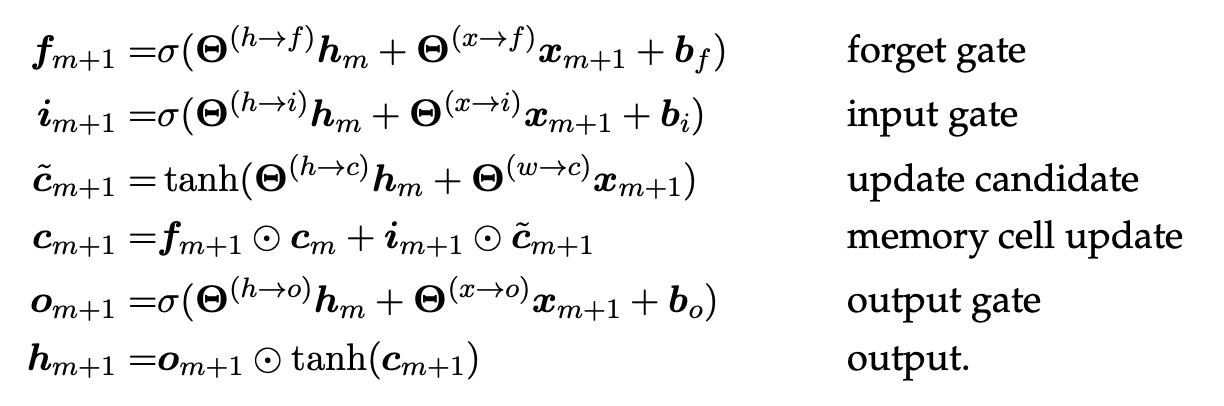
\includegraphics[width=0.8\textwidth]{Images/midterm_images/lstm.png}
    \caption{LSTM update equations (Eisenstein Ch. 6.33).}
    \label{fig:lstm}
\end{figure}

The update equations for a LSTM at timestep $m+1$ are given in \autoref{fig:lstm}. Eisenstein Chapter 6.3 may be useful in answering this question. 

\begin{enumerate}

\begin{table}[h!]
    \centering
    \begin{tabular}{|cc|}
    \toprule
    \textbf{Weight} & \textbf{Value} \\
    \midrule
    $\boldsymbol{\Theta}^{(h\rightarrow f)}$ & $[1,-2,-3]^T$ \\
    $\boldsymbol{\Theta}^{(x\rightarrow f)}$ & $[0,-1,-2]^T$ \\
    $\boldsymbol{b}_f$ & $0$ \\
    $\boldsymbol{\Theta}^{(h\rightarrow i)}$ & $[0,0,1]^T$\\
    $\boldsymbol{\Theta}^{(x\rightarrow i)}$ & $[-1,-2,-2]^T$\\
    $\boldsymbol{b}_i$ & $1$ \\
    $\boldsymbol{\Theta}^{(h\rightarrow c)}$ & $\begin{bmatrix}
    0 & 1 & -3\\
    -3 & 1 & 0\\
    -2 & -1 & -3
        \end{bmatrix}$ \\
    $\boldsymbol{\Theta}^{(w\rightarrow c)}$ & $\begin{bmatrix}
    1 & 0 & 0 \\
    -2 & -3 & 0\\
    1 & -1 & -2 \end{bmatrix}$ \\
    $\boldsymbol{\Theta}^{(h\rightarrow o)}$ & $[1,0,1]^T$\\
    $\boldsymbol{\Theta}^{(x\rightarrow o)}$ & $[-1,0,1]^T$\\
    $\boldsymbol{b}_o$ & $-1$ \\
    \bottomrule
    \end{tabular}
    \caption{Weights for LSTM.}
    \label{tab:lstm_weights}
\end{table}

\item In \autoref{tab:lstm_weights} we provide weight values and in \autoref{tab:lstm_intvars} timestep inputs. We'll now compute the value of $\boldsymbol{h}_{m+1}$ using \autoref{tab:lstm_weights} and \autoref{tab:lstm_intvars}: 

\begin{table}[h!]
    \centering
    \begin{tabular}{|cc|}
    \toprule
    \textbf{Vector} & \textbf{Value} \\
    \midrule
    $\boldsymbol{h}_m$ & $[3,1,-1]^T$ \\
    $\boldsymbol{c}_m$ & $[1,0,-4]^T$ \\
    $\boldsymbol{x}_{m+1}$ & $[-3,-2,-1]^T$ \\
    \bottomrule
    \end{tabular}
    \caption{Input/intermediate variables for LSTM.}
    \label{tab:lstm_intvars}
\end{table}

$\boldsymbol{f}_{m+1} = \sigma(4 + 4 + 0) = 1.0$ \\
\indent $\boldsymbol{i}_{m+1} = \sigma(-1 + 9 + 1) = 1.0$ \\
\indent $\boldsymbol{\tilde{c}}_{m+1} = \text{tanh}([4, -8, -4]^T + [-3, 12, 1]^T) = \text{tanh}([1,4,-3]^T) = [0.76, 1.0, -1.0]^T$\\
\indent $\boldsymbol{c}_{m+1} = 1.0 \odot [1,0,-4]^T + 1.0 \odot [0.76, 1.0, -1.0]^T = [1.76, 1.0, -5.0]^T $ \\
\indent $\boldsymbol{o}_{m+1} = \sigma(2 + 2 - 1) = 1.0$\\
\indent $\boldsymbol{h}_{m+1} = 1.0 \odot \text{tanh}([1,0,-4]^T) = \mathbf{[0.76, 0, -1.0]^T}$\\

The gates of this LSTM do not restrict the flow of any information. To effectively turn this LSTM into an Elman RNN at the current timestep, i.e., include \textbf{only} information from the current input and prior hidden state and \textbf{no} information from the prior memory cell in $\boldsymbol{h}_{m+1}$, describe the values that you would need to set the gates $\boldsymbol{f}_{m+1}, \boldsymbol{i}_{m+1}$ and $\boldsymbol{o}_{m+1}$ equal to.

\item Which variable from the list of intermediate variables in \autoref{fig:lstm}, \autoref{tab:lstm_weights} most closely resembles the hidden state of a standard Elman RNN? (Answer choices are $\boldsymbol{f}_{m+1}$, $\boldsymbol{i}_{m+1}$, $\boldsymbol{\tilde c}_{m+1}$, $\boldsymbol{c}_{m+1}$, $\boldsymbol{o}_{m+1}$, $\boldsymbol{h}_{m+1}$).

\item In this problem, all the LSTM gates are scalars. What changes would have to be made to \autoref{tab:lstm_weights} in order to create vector gates? (Specify which weights would change and what their new dimensions would be). What is the benefit of vector gates over scalars?

\item What two problems in RNNs does the inclusion of the memory cell $\boldsymbol{c}_{m+1}$ improve? What property of its computation allows it to do this?

\end{enumerate}


\section{Beam Search Decoding}
Consider the following bigram language model. The bigram probabilities are given in table \ref{tab:bigram_prob}. Each probability is of the form $P(x_i|x_{i-1})$, where $x_i$ corresponds to $i^{th}$ word in a post / word sequence. Here, $\langle s \rangle$ denotes the start of a sentence.

\begin{table}[h!]
    \centering
    \begin{tabular}{|l|c|l|c|}
    \toprule
        Bigram & Prob. & Bigram & Prob.\\
        \hline
        P(, $|$ know) & 0.4 & P(important $|$ the) & 0.3 \\
        P(the $|$ know) & 0.6 & P(response $|$ correct) & 0.6 \\
        P(I $|$ ,) & 0.8 & P(answer $|$ correct) & 0.25  \\
        P(it $|$ ,) & 0.2 & P(problems $|$ correct) & 0.15  \\
        P(will $|$ I) & 0.4 & P(response $|$ important) & 0.5 \\
        P(know $|$ I) & 0.6 & P(answer $|$ important) & 0.5\\
        P(was $|$ it) & 1.0 & P(answer $|$ exact) & 1.0 \\
        P(correct $|$ the) & 0.5 &  P(exact $|$ the) & 0.2 \\
    \bottomrule
    \end{tabular}
    \caption{Bigram Language Model probabilities for Beam Search.}
    \label{tab:bigram_prob}
\end{table}

\begin{enumerate}
    \item Given a prefix string ``$\langle s\rangle\;I\;know$'', what are the next $3$ possible tokens. Run beam search with width $k=2$ and generate the next $3$ tokens. 
    
    Assume $P(\langle s  \rangle\;I\;know) = 1$. Make sure you show the probabilities for each step. Also, show the word sequences in the beam at the end of each step.
    
    \item Lets introduce some randomness into the standard beam search method used in question $3.1$. At the end of each step, we randomly choose one of the top-k beam candidates and discard the rest. In other words, only the randomly chosen top-k candidate is expanded in the next step instead of all the top-k candidates. Figure \ref{fig:top_k} illustrates this sampling approach.
    
    \begin{figure}[h!]
    \centering
    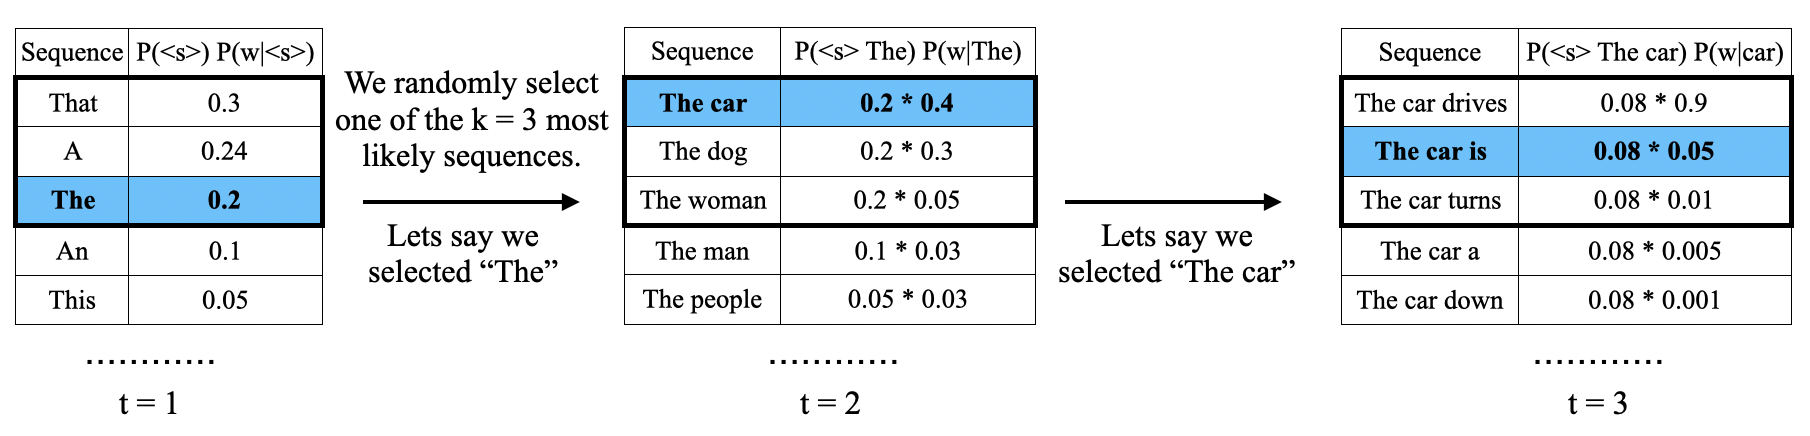
\includegraphics[width=0.92\textwidth]{Images/midterm_images/top_k_sampling.png}
    \caption{Example of top-k random sampling. At each timestep t, the model generates the probability of the possible next word. Then, we randomly sample from the $k$ most likely candidates from this distribution. Here, we consider $k = 3$. \textbf{Bold} sequences represent the sampled candidate at each timestep.}
    \label{fig:top_k}
\end{figure}
    
    Once again, consider the bigram language model in Table \ref{tab:bigram_prob}.
    
    \begin{enumerate}
        \item Given the prefix string ``$\langle s\rangle\;I\;know$'', run the top-k sampling approach for the next 3 tokens.  Let $S$ be the set of output sequences that this approach could possibly generate at the end of 3 steps. What is the size of $S$? Assume $k = 2$ and $P(\langle s  \rangle\;I\;know) = 1$. You can just report the number.
        
        \item What is the sequence with maximum probability in $S$? Report the sequence and the probability of the sequence. 
        
        \item What is the sequence with  minimum probability in $S$? Report the sequence and the probability of the sequence.
        
    \end{enumerate}

\end{enumerate}

\section{Evaluation}

\begin{enumerate}

    \item Consider the following sentence with gold and predicted named entity tags.
    
    
    \begin{table}[h!]
    \begin{center}
    \small
    \begin{tabular}{l} 
    \hline
    \textbf{Predicted NER Tags} \\
    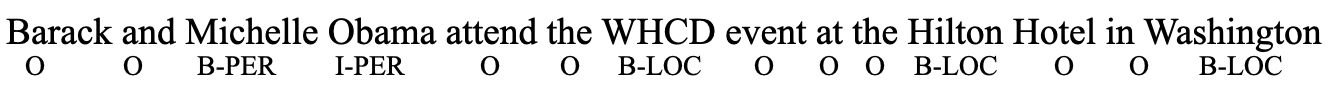
\includegraphics[scale=0.5]{Images/midterm_images/predicted_tags.png}
    \\
    \hline
    \textbf{Gold NER Tags} \\
    
\includegraphics[scale=0.5]{Images/midterm_images/gold_tags.png}
    \\
    \hline
    \end{tabular}
    \caption{Predicted and gold NER tag sequences.}
    \end{center}
    \end{table}

    
  Compute the overall precision, recall, and F1 scores for the predicted entity tag sequence. Assume that the prediction is correct only when there is an exact match between the predicted entity span and the gold span. 
    
    \item 
    
    $BLEU$ score is the most common automatic evaluation metric for machine translation. Given a candidate translation $\mathbf{c}$ and human-written reference translations $\mathbf{r_1}, . . . , \mathbf{r_k}$, we compute the $BLEU$ score of $\mathbf{c}$ as follows:
    
    We first compute the modified n-gram precision $p_n$ of $\mathbf{c}$ with $n = 1,2,3,4$. Here $n$ is the size of ngram:
    
    \begin{align*}
        p_n = \frac{\sum_{ngram \in c} min \Big( Max\_Ref\_Count(ngram), Count_{c}(ngram) \Big) }{\sum_{ngram \in c} Count_{c}(ngram)} \\
        Max\_Ref\_Count(ngram) = max_{i=1..k} Count_{r_i}(ngram) 
    \end{align*}
    
    For each of the n-grams in $\mathbf{c}$, we count the maximum number of times it appears in any one reference translation. Then, we clip this count by the number of times it appears in $\mathbf{c}$. We divide these clipped counts by the number of ngrams in $\mathbf{c}$.
    
    Next, we compute the brevity penalty $BP$. Let $len(\mathbf{c})$ be the length of $c$ and let $len(\mathbf{r})$ be the length of the shortest reference translation.
    
    \begin{equation*}
    BP =  
    \begin{cases}
        1 & \text{if } len(\mathbf{c}) \geq len(\mathbf{r})\\
        exp(1 - \frac{len(\mathbf{r})}{len(\mathbf{c})}) & \text{otherwise}
    \end{cases}
    \end{equation*}

    Lastly, the $BLEU$ score for candidate $c$ with respect to $r_1, . . . , r_k$ is:
    
    \begin{equation}
        BLEU = BP\;\exp(\sum_{n=1}^{N} w_n \log p_n)
    \end{equation}

    where $w_1 , w_2 , w_3 , w_4$ are weights that sum to 1. The log here is natural log.
    

    Compute the $BLEU$ score for the following two candidate translations $\mathbf{c_1}, \mathbf{c_2}$ against two human-written references $\mathbf{r_1}, \mathbf{r_2}$:
    
    \begin{description}
            \item Candidate Translation $\mathbf{c_1}$: fruits are good for health
            \item Candidate Translation $\mathbf{c_2}$ vegetables are very important for good health
            \item Reference Translation $\mathbf{r_1}$: eating fruits is good for health
            \item Reference Translation $\mathbf{r_2}$: fruits and vegetables are essential for good health
    \end{description}
        
    Let $w_i = \frac{1}{3}$ for $i \in {1,2,3}$ and $w_4 = 0$. In other words, we do not compute 4-grams. Show the computation of $p_1$, $p_2$, $p_3$, $BP$, and the final $BLEU$ score in your answer.

\end{enumerate}

\section{HMM}

Consider the problem of POS Tagging using Hidden Markov Models. Assume that our vocabulary only contains the words "Paul's", "red", "pen", and "leaked". There are only 3 states corresponding to the tags Proper Noun(PN), Noun(N), and Not Noun(NN). The parameters of the HMM model are as follows:

\begin{table}[h!]
\begin{center}

\begin{tabular}{ |c|c|c|c| } 
\hline
 & PN & N & NN \\
\hline
$\pi$ & 0.1 & 0.3 & 0.6 \\ 
\hline
\end{tabular}
\caption{Initial probabilities}
\end{center}
\end{table}

\begin{table}[h!]
\begin{center}
\begin{tabular}{ |c|c|c|c| } 
\hline
from/to & PN & N & NN \\
\hline
PN & 0   & 0.2 & 0.8 \\
N  & 0.1 & 0   & 0.9 \\
NN & 0.2 & 0.4 & 0.4 \\
\hline
\end{tabular}
\caption{Transition probabilities}
\end{center}
\end{table}

\begin{table}[h!]
\begin{center}
\begin{tabular}{ |c|c|c|c|c| } 
\hline
 & Paul's & red & pen & leaked \\
\hline
PN & 0.7 & 0.2 & 0.1 & 0 \\
N  & 0.1 & 0.2 & 0.6 & 0.1 \\
NN & 0   & 0.4 & 0.1 & 0.5 \\
\hline
\end{tabular}
\caption{Emission probabilities for the states PN, N, and V}
\end{center}
\end{table}

\newpage

\begin{enumerate}
    \item Compute the probability of the observed sequence "Paul's red pen leaked" by using the Forward Algorithm on the given HMM model.

    \item Use the viterbi algorithm on the given HMM model to determine the best sequence of tags for the sentence "Paul's red pen leaked" and the probability of that sequence of tags. If there are ties, break them in this order  NN $<$ N $<$ PN. 

    \item What is the time complexity of the Viterbi Algorithm in terms of the number of possible labels (Y) and the sequence length (T)? Justify your answer. 

\end{enumerate}

\section{Transformer Self Attention}
This section deals with transformer self attention. It may be helpful to read section 9.7 in the Speech and Language Processing textbook while answering these questions. \textbf{For all questions in this section, unless otherwise stated work must be shown in the form of matrix multiplications to receive full credit} (i.e. $C = AB^T$). For performing the computations, using Excel or other software is recommended to avoid computation errors. When writing your answers please round to 2 decimal places. You may use scientific notation to represent your answers if necessary.
\begin{enumerate}

\begin{table}[H]
\begin{center}
\begin{tabular}{ |c|c|c|c| } 
\hline
 Word &  \multicolumn{3}{c|}{}   \\
\hline
Attention & 1  & 2  & 4  \\
is        & -1  & 0  & 2  \\
all       & 3   & 1  & 3  \\
you       & 5   & 0  & 0  \\
need      & 2   & -2 & -1 \\
\hline
\end{tabular}
\caption{Word embeddings}
\end{center}
\end{table}

\[
W^q = 
\begin{bmatrix}
    1   &  1      \\
    -3  &  1      \\
    -2  &  3      
\end{bmatrix}
,\ W^k = 
\begin{bmatrix}
    -1  &  3      \\
    -2  &  -5      \\
    -1  &  -2      
\end{bmatrix}
,\ W^v = 
\begin{bmatrix}
    3  &  0      \\
    2  &  -4      \\
    4  &  -0      
\end{bmatrix} 
\]

\[
W^o = 
\begin{bmatrix}
     -5  &  4    &  -5  \\
     2   &  -1   &  2   \\
     1   &  -4   &  4   \\
     0   &  0    &  0   \\
     3   &  3    &  -1  \\
     -4  &  -3   &  -1  \\
     3   &  1    &  5   \\
     1   &  3    &  3  
\end{bmatrix}
\]


 \item We will first consider a single attention head. Given the set of word embeddings, projection matrices, and a normalization factor of $48$ instead of $\sqrt{d^k}$, fill out this table with the normalized query-key score for each possible pair of words.


\begin{table}[H]
\begin{center}
\begin{tabular}{ |c|c|c|c|c|c| } 
\hline
 Word  &  \multicolumn{1}{c}{} \hspace{0.5cm}  & \multicolumn{1}{c}{} \hspace{0.5cm}  & \multicolumn{1}{c}{} \hspace{0.5cm}  &  \multicolumn{1}{c}{}\hspace{0.5cm}  &  \hspace{0.5cm}  \\
\hline
Attention &    &   &   &   &  \\
\hline
is        &    &   &   &   &  \\
\hline
all       &    &   &   &   &  \\
\hline
you       &    &   &   &   &  \\
\hline
need      &    &   &   &   &  \\
\hline
\end{tabular}
\caption{Normalized Scores}
\end{center}
\end{table}

\item Given the normalized scores, calculate the attention weights for each word with respect to the other words in the input sentence and fill in the table with your results. You do not need to show work for this question.

\begin{table}[H]
\begin{center}
\begin{tabular}{ |c|c|c|c|c|c| } 
\hline
 Word  &  \multicolumn{1}{c}{} \hspace{0.5cm}  & \multicolumn{1}{c}{} \hspace{0.5cm}  & \multicolumn{1}{c}{} \hspace{0.5cm}  &  \multicolumn{1}{c}{}\hspace{0.5cm}  &  \hspace{0.5cm}  \\
\hline
Attention &    &   &   &   &  \\
\hline
is        &    &   &   &   &  \\
\hline
all       &    &   &   &   &  \\
\hline
you       &    &   &   &   &  \\
\hline
need      &    &   &   &   &  \\
\hline
\end{tabular}
\caption{Attention Values}
\end{center}
\end{table}

\item Given the embeddings, the previously calculated attention values, and the value projection matrix, calculate the output embeddings of this attention head. Fill in the table with your results. 

\begin{table}[H]
\begin{center}
\begin{tabular}{ |c|c|c| } 
\hline
 Word  &  \multicolumn{1}{c}{} \hspace{0.5cm}  &   \hspace{0.5cm}  \\
\hline
Attention &    &   \\
\hline
is        &    &  \\
\hline
all       &    &   \\
\hline
you       &    &   \\
\hline
need      &    &   \\
\hline
\end{tabular}
\caption{Self Attention Head Outputs}
\end{center}
\end{table}

\item The outputs of three other self attention heads have been computed for you. Combine these values with the self attention embedding you calculated earlier in this question, and find the final output of this self attention layer using the output weight matrix. Fill in the table with your results.

\begin{table}[H]
\begin{tabular}{ |c|c|c| } 
\hline
 Word  &  \multicolumn{1}{c}{} \hspace{0.5cm}  &   \hspace{0.5cm}  \\
\hline
Attention &  1.5    & -2.5   \\
\hline
is        & -4.78   & 0.15 \\
\hline
all       & 1.75    & -1.97  \\
\hline
you       & -3.96   & -2.9  \\
\hline
need      & -0.53   &  4.61 \\
\hline
\end{tabular}
\hfill
\begin{tabular}{ |c|c|c| } 
\hline
 Word  &  \multicolumn{1}{c}{} \hspace{0.5cm}  &   \hspace{0.5cm}  \\
\hline
Attention & 1.51   & 0.07   \\
\hline
is        & -4.95  & -3.47 \\
\hline
all       & 2.33   & -4.81  \\
\hline
you       & 0.05   & 0.68   \\
\hline
need      & 2.85   & -1.91  \\
\hline
\end{tabular}
\hfill
\begin{tabular}{ |c|c|c| } 
\hline
 Word  &  \multicolumn{1}{c}{} \hspace{0.5cm}  &   \hspace{0.5cm}  \\
\hline
Attention &  -3.59  & -3.18  \\
\hline
is        &  3.38   & -1.85 \\
\hline
all       &  3.77   & 4.21  \\
\hline
you       &  -0.15  & 1.46  \\
\hline
need      &  -1.65  & 1.51  \\
\hline
\end{tabular}
\caption{Other Attention Head Outputs}
\end{table}

  \begin{table}[H]
\begin{center}
\begin{tabular}{ |c|c|c|c| } 
\hline
 Word &  \multicolumn{1}{c}{} \hspace{0.5cm} & \multicolumn{1}{c}{} \hspace{0.5cm} & \hspace{0.5cm} \\
\hline
Attention &   &   &   \\
\hline
is        &   &   &   \\
\hline
all       &   &   &   \\
\hline
you       &   &   &   \\
\hline
need      &   &   &   \\
\hline
\end{tabular}
\caption{Output of self attention layer}
\end{center}
\end{table}
 
  \item Given your understanding of the differences between recurrent networks and transformers, why do transformers tend to outperform recurrent networks in terms of computational efficiency? (1-2 sentences)
 
\end{enumerate}





\section{Extra Credit}

For this open-ended question, we will ask you to help find some data for a research project. 

\begin{enumerate}
    \item Users on the Internet sometime may willingly or accidentally reveal information about themselves. Please find at least five posts on Reddit (\url{https://www.reddit.com/}) where users revealed information about themselves (\textbf{other than age or gender}). List the URL of the Reddit posts, the sentence(s) in each post where the user disclosed information about themselves, and the type(s) of information that was disclosed. 
    
    \item How did you find these posts? Explain the strategy you used. 
    
    \item Any thoughts or interesting observations you have as you search for these posts?

\end{enumerate}



\end{document}

